\section{Aufgabe 2}
\label{sec:Aufgabe2}
\subsection{Teil a)}
Da bei der Poissonverteilung sowohl der Mittelwert als auch die Varianz
durch $\lambda$ gegeben
ist, wählen wir für die Gaußverteilung $\mu=\lambda$ und $\sigma^2=\lambda$.
Da ich nicht weiß, wie ich das beweisen soll, habe ich ein Paar Beispielplots gemacht.
\begin{figure}[H]
  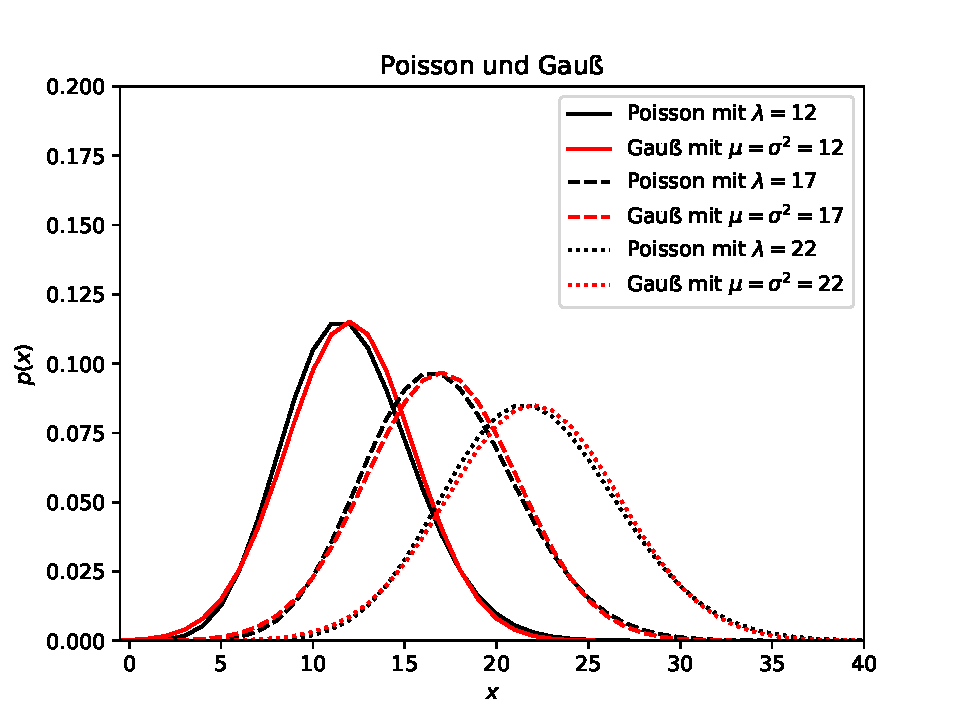
\includegraphics{plots/testplot.pdf}
  \caption{Beispielplots der Gauß- und Poissonverteilung mit drei
            unterschiedlichen $\lambda$.}
\end{figure}
Das sieht doch ganz ähnlich aus.
\subsection{Teil b)}
Kolmogorow–Smirnow-Test wurde wie in der Vorlesung beschreiben implementiert.
\subsection{Teil c) und d) }
Es wurden für die Konfidenzniveaus $\alpha = 0,05 $ , $ \alpha = 0,025 $ und $ \alpha = 0,001 $
alle ganzzahligen $\lambda \in [1,15]$ getestet. \\
Für $\alpha = 0,05$ kann der Kolmogorow–Smirnow-Test ab $\lambda=8$ nicht mehr unterscheiden.\\
Für $\alpha = 0,025$ kann der Kolmogorow–Smirnow-Test für $\lambda=6$ nicht mehr unterscheiden,
dann für $\lambda=7$ gehts wieder und ab $\lambda=8$ dann nicht mehr. Ich nehme an das liegt
an den gezogenen Zufallszahlen.\\
Für $\alpha = 0,001$ kann der Kolmogorow–Smirnow-Test ab $\lambda=5$ nicht mehr unterscheiden.
